% Chapter Analysis Strategy

\chapter{Analysis Strategy} \label{Analysis Strategy}

The target of the analysis is to search for the heavy resonances decaying to di-Higgs whose mass is above 800 GeV. Each Higgs boson is assumed to further decay to ${b\bar{b}}$ and is reconstructed in a lareger boosted jet including two b-flavored-like merged sub-jets by anti-kT08 algorithm. Higgs identification is done by selection on soft-drop PUPPI mass, n-subjetness, and double b-tagger. 

\hypersetup{colorlinks,linkcolor=black,urlcolor=black}
\section{Data and Simulated Samples} \label{Data and simulated samples}
The analysis is preformed based on the data collected in pp collision with the CMS detector at $\sqrt{s}$ = 13 TeV. The integrated luminosity is 35.9$fb^{-1}$. Runs in which the detector normally operates was chosen according to the golden JSON file: $\href{https://cms-service-dqm.web.cern.ch/cms-service-dqm/CAF/certification/Collisions16/13TeV/ReReco/Final/Cert_271036-284044_13TeV_23Sep2016ReReco_Collisions16_JSON.txt}{Cert\_271036-284044\_13TeV\_23Sep2016ReReco\_Collisions16\_JSON.txt}$. The samples of data is listed in Table 1. 

\begin{table}[h!]
  \begin{center}
    \begin{tabular}{l|l|l}
    Dataset & Processing & Int. lumi. ($fb^{-1}$) \\
    \hline
    JetHT/Run2016B & 23Sep2016 & 5.9\\
    JetHT/Run2016C & 23Sep2016 & 2.6\\
    JetHT/Run2016D & 23Sep2016 & 4.4\\
    JetHT/Run2016E & 23Sep2016 & 4.1\\
    JetHT/Run2016F & 23Sep2016 & 3.2\\
    JetHT/Run2016G & 23Sep2016 & 7.7\\
    JetHT/Run2016H & PromptReco & 8.9\\
    \hline
    Total & & 35.9\\
    \end{tabular}
  \end{center}

  \caption{List of datasets used in the analysis and its corresponging integrated luminosity in pp collision at $\sqrt{s}$ = 13 TeV.}
\end{table} 

\section{Monte Carlo Simulation} \label{Monte Carlo Simulation}	

\section{Triggers} \label{Triggers}
Since the final state includes di-Higgs jet, the trigger are selected considerring the requirements from the scale sum of external energy $H_T$, |$\Delta \eta $| and mass of dijet, jet transverse momentum $p_T$, the jet groomed mass, and b-tagger. PFHT900 is used to supplement the inefficiency of PFHT800 in period H of data taking.
\begin{table}[h!]
  \begin{center}
    \begin{tabular}{l}
    Triggers \\
    \hline
    HLT$\_$PFHT800 \\
    HLT$\_$PFHT900 \\
    HLT$\_$PFHT650$\_$WideJetMJJ900DEtaJJ1p5 \\
    HLT$\_$AK8PFJet360$\_$TrimMass30 \\
    HLT$\_$AK8DiPFJet280$\_$200$\_$TrimMass30$\_$BTagCSV$\_$p20 \\
    HLT$\_$AK8PFHT650$\_$TrimR0p1PT0p03Mass50 \\
    \hline
    \end{tabular}
  \end{center}

  \caption{List of Triggers applied in the analysis.}
\end{table} 


\section{Event Reconstruction and Selection} \label{Event reconstruction and selection}
%MET Filters & AND \\
%https://twiki.cern.ch/twiki/bin/view/CMS/MissingETOptionalFiltersRun2#How_to_run_the_Bad_Charged_Hadro 
To reduce the impact from both cosmic particles and noise of calorimeters, missing transverse energy, MET, filters are applied.
If all particles are detected and well-reconstructed in the detector, the sum of transverse momentum will be zero. However, if there is noise or ill-reconstructed particles or jets, the sum of transverse momentum will not equal to zero, and the negative of its value is defined as MET.  
The filters remove most events having anomaly MET based on different information given from the detectors.
\begin{table}[h!]
  \begin{center}
    \begin{tabular}{l}
    Triggers \\
    \hline
    primary vertex filter\\
    beam halo filter\\
    HBHE noise filter\\
    HBHE iso noise filter\\
    ECAL TP filter\\
    ee badSC noise filter\\
	Bad PF Muon Filter\\
	Bad Charged Hadron Filter\\ 
    \hline
    \end{tabular}
  \end{center}

  \caption{List of MET filters applied in the analysis.}
\end{table}

%Number of good vertex & $>$1 \\
After passing MET filters, at least one reconstructied pp collision vertex is required in an event, which should pass following criteria:
\begin{itemize}[noitemsep]
\item Number of degree of freedom $>$ 4
\item Absolute displacement from the beamspot position along the z direction $<$ 24 cm
\item Absolute displacement from the beamspot position along the transverse direction $<$ 2 cm
\end{itemize}


%Lepton veto & one tight-tagged or two opposite charged loose-tagged \\
For the final state is all-hadronic, lepton veto is implemented. The event will be veto either there is single tight-tagged muon or electron, or there are two loose-tagged opposite charged mouns or electrons.

\subsection{Higgs Jet Reconstruction} 
%http://iopscience.iop.org/article/10.1088/1126-6708/2008/04/063/pdf
%http://cds.cern.ch/record/1194487
%http://cds.cern.ch/record/1247373
Each candidate of particles is reconstructed with Particle-Flow, PF, algorithm in CMS by all the detector components which priority form high to low: muons, electrons, photons, charged hadrons, and neutral hadrons.

The jets are clustered with anti-$k_{T}$ algorithm by PF candidates. Anti-$k_{T}$ algorithm is done desribed below: 
\begin{equation} \label{eq1}
\begin{split}
d_{ij} = min(k^{2p}_{ti},k^{2p}_{tj})\dfrac{\Delta ^2_{ij}}{R^2}\\
d_{iB} = k^{2p}_{ti} ,	
\end{split}
\end{equation}

where $\Delta ^{2p}_{ij}= (y_{i}-y_{j})^2+(\phi_{i}-\phi_{j})^2$ and $k_{ti}$, $y_{i}$, and $\phi _{i}$ are the transverse momentum, rapidity, and azimuthof particle i.
Considering minimum term between one hard particle and one soft particle compared to that between the soft particle and another soft particle, the former will be smaller because transverse momentum of hard particle is larger, while its inverse square is smaller. 
Therefore, $d_{ij}$ of the former is shorter, that is, a soft particle is more likely to cluster with hard particle around it. 
As a consequence, if there is no other hard particle within the range 2R of the hard particle, it will cluster a conical jet with all soft particles within range R. 
In other situation where R $<$ distance of two hard particles $<$ 2R, one can show that the particle having larger transverse momentum will have conical, while another is partly conical.
Last, where distance of two hard particles $<$ R, two particles will merge into single jet. The jets is clustered using range parameter R set to 0.8 (refrred to AK8 jets).

%https://arxiv.org/pdf/1407.6013.pdf
In one bunch crossing, the vetex having highest energy called primary vertex, and the others are called Pile-ups, PUs. PUs may contribute some components in jets which does not origninally belong to them. We can mitigate the effect by PUPPI algorithm, which will be descripted below:
 A shape $\alpha _{i}$ for a given particle i is defined: 
\begin{equation} \label{eq2}
\begin{split}
\alpha_i = log \sum\limits_{j\in event} \xi _{ij} \times \Theta(\Delta R_{ij} - R_{min}) \times \Theta(R_0 - \Delta R_{ij}) \\
\xi _{ij} = \dfrac{p_{Tj}}{\Delta R_{ij}}
\end{split}
\end{equation}
where $\Theta$ is the Heaviside step function, $p_{T}$ is the transverse momentum, and $\Delta R_{ij}$ is the distance between particle i and j in $\eta \phi$ space. Hence, only particles fall in the cone size $R_0$ but not closer than $R_{min}$ contribute to $\alpha $. $R_0$ represent the locality of a jet, and $R_{min}$ is mainly restricted by resolution of the detector. Then we seperate events into two cases: with and without tracker information. The former is used to weight the charged particles in central region, while the latter is used for charged particles in forward region and neutral particles with an addition rapidity factor applied to forward region. The calculation of weight uses the quantities of median and the left-side RMS of $\alpha $ distibution. Finally, the weight of an particle will be: 
\begin{equation} \label{eq3}
\begin{split}
\chi ^2_{i} = \Theta(\alpha _i - \bar{\alpha } _{PU}) \frac{ ( \alpha _i - \bar{\alpha } _{PU})^2 }{\sigma ^2 _{PU}} , \\
\omega _i = F_{\chi ^2,NDF=1}(\chi ^2_i) 
\end{split}
\end{equation}
,where $F_{\chi ^2}$ is the cumulative distribution function of the $\chi ^2$ distribution. One can find that if $\alpha $ of a particle less than the median, it will be considered from PU, and the step function in the first eqation gives it a value of zero, while if it greater than the median, the value of $\chi $ is close to one. 

%$p_{T}$ of Higgs jets & $>$300GeV \\
%|$\eta$| of Higgs jets & $<$2.4 \\
%Tight LepVeto jet ID & 1 \\
Basic selection is applied on AK8 jet. We only consider the jets having the largest and the second largest transverse momentum in an event. The $p_{T}$ of the jets must greater than 300 GeV and pseudorapidity |$\eta$| must less than 2.4. Also, the tight PF jet identification provided by JETMET group is required, which is summarized in the table, where fraction are referring to energy fraction, and constituents and multiplcity are referring to the number of particles.
%to-do table number 
%https://twiki.cern.ch/twiki/bin/viewauth/CMS/JetID#Recommendations_for_13_TeV_2016

\begin{table}[h!]
  \begin{center}
    \begin{tabular}{ll}
    Variable & Cut \\
    \hline
    Neutral hadron fraction & $<$0.9 \\
    Neutral EM fraction & $<$0.9 \\
    Charged EM fraction & $<$0.9 \\
    Number of Constituents & $>$1 \\
    Muon fraction & $<$0.8 \\
    Charged hadron fraction & $>$0 \\
    Charged Multiplicity & $>$0 \\
	\hline
    \end{tabular}
  \end{center}

  \caption{List of Triggers applied in the analysis.}
  \end{table}

\subsection{Heavy Resonance Seletion} 
Because of the difference between the mass of heavy resonanace and the Higgs jets, the difference between two |$\eta $| of jets of the signal events will be less than that of multi-jet events. To reduce the contribution from multi-jet events, our mainly source of background, we require a |$\Delta \eta $| cut on $<$ 1.3. 
%|$\Delta \eta (two Higgs jets)$| & $<$1.3 \\
We targeted the heavy resonances whose mass is above 800 GeV. Therefore, a requirement is used on a revised mass of heavy resonances. The mass of heavy resonances, $M_{jj}$, is get from addition of four momentum of two Higgs jets. A revised mass is used to improve the resolution and correct the peak position of the $M_{jj}$ distribution, referred as "reduced mass" for the following chapters.
\begin{equation} \label{eq4}
\begin{split}
M^{reduced}_{jj} = M_{jj} - (M_{j1} - M_{H} ) - (M_{j2} - M_{H} )
\end{split}
\end{equation}

,where $M_{j1}$ or $M_{j2}$ is the mass of Higgs jets, and $M_{H}$ is the mass of physic Higgs boson. Reduce mass must greater than 750 GeV. 
%Reduce mass & $>$750 GeV \\

\subsection{Higgs Tagging Seletion} 

%http://xxx.lanl.gov/pdf/1402.2657v2
%CMS Collaboration, “Search for heavy resonances in the W/Z-tagged dijet mass spectrum at 13 TeV”, CMS Analysis Note CMS-AN-16-235, CERN, 2016.
%PUPPI soft-drop mass with W boson generator level correction & 105$<$ and $<$135 \\
The soft-drop procedure is inplemented to re-cluster the jet by removing soft contribution as follow:
\begin{itemize}
\item Deculster a targeted jet into two sub-jets.
\item Continue to decompose the sub-jets until the condition is achieved
\begin{equation} \label{eq5}
\begin{split}
\frac{min(p_{T1},p_{T2})}{p_{T1}+p_{T2}} > Z_{cut} \times (\frac{\Delta R_{12}}{R_0})^{\beta}
\end{split}
\end{equation}
, where $R_0$ is the cone size of the original cluster algorithm, $p_T$ are the transverse momenta of two sub-jets, $\Delta R_{12}$ is the distance of two sub-jets in $\eta \phi$ space, and $Z_{cut}$ and $\beta $ are parameters. 
\item The unsplit singelet particle at the end will either be removed or remain preserved.
\end{itemize} 
If $\beta  >$ 0, the soft contribution is removed while remain a fraction of soft-clooinear radiation. 
If $\beta  <$ 0, soft drop removes both  soft and collinear radiation.
In CMS, the $Z_{cut}$ and $\beta $ are set 0.1 and zero respectively.
The difference of the peak of the distribution of mass of PUPPI soft-drop jets and the physical mass is found.
A Correction is applied to move the peak to the true phyiscal value. 
The ratio is derived by mass of peak of reconstruction jets to mass of true physical mass from WW dijet Monte Carlo simulations.
The corrected PUPPI soft-drop mass of the first two leading jets are required between 105 and 135 GeV which has been optimized.
 
%https://arxiv.org/abs/1011.2268
%https://arxiv.org/pdf/1108.2701
%https://arxiv.org/abs/1004.2489
%https://twiki.cern.ch/twiki/bin/view/CMS/JetWtagging#Working_points_and_scale_factors
%$\tau$21 & $<$ 0.55 \\
The $\tau _N $ to $\tau _{N-1}$ ratio is used as a discriminant to seperate the boosted events decaying into N particles from QCD multijet events where $\tau _N $ is so-called "N-subjettiness" algorithm:
\begin{equation} \label{eq6}
\begin{split}
\tau _N = \frac{1}{d_0} \sum\limits_{k}  p_{T,k} min \{ \Delta R_{1,k},\Delta R_{2,k},\cdots,\Delta R_{N,k} \} \\
d_0 = \sum\limits_{k}  p_{T,k} R_0,
\end{split}
\end{equation}
where k runs over the constituent particles in a given jet, $\Delta R_{jk}$ is the distance between particle j and k in $\eta \phi$ space, $R_0$ is the cone size of the original cluster algorithm. In the analysis boosted jets are decaying into two sub-jets, so $\tau _2 $ to $\tau _1$ ratio is used.
The $\tau _2 $ to $\tau _1$ ratio is required to be less than 0.55.  
The working point and simualtion to data scale factor is derived by JME POG.

The double-b tagger is a multiple varialbe analysis discriminant used to identify b-flavor jets. hets in QCD evetns and Higgs jets decaying into bb are used for training. Here lists out the input information:
\begin{itemize}
\item The first four impact paramters to its uncertainties values ordered from the largest to the smallest.
\item The  N-subjettiness axes referred as $\tau $-axes use the information of N-subjettiness and the first two impact paramters to its uncertainties values of $\tau $-axes ordered from the largest to the smallest.
\item The meausured significance of impact parameters of the first two tracks whose secondary vertex is above buttom quark threshold.
\item The number of secondary vertex of the jet.
\item The significance of two dimenisional distance between primary vertex and secondary vertex and flight distance of secondary vertex with smallest three dimenisional distance uncertainty for each $\tau $-axes.
\item $\Delta R$ of two secondary vertex with smallest three dimenisional distance uncertainty for each $\tau $-axes.
\item The $\tau $-axis of two secondary vertex with smallest three dimenisional distance uncertainty for each $\tau $-axes.
\item The total of mass of secondary vertex associated to the $\tau $-axis for each $\tau $-axes.
\item The relative pseudorapidity of three tracks of leading secondary vertex with respect to their $\tau $-axis for each $\tau $-axes.
\item The total of energy of secondary vertex associated to the $\tau $-axis for each $\tau $-axes.
\item The total of energy of all tracks in the Higgs jet (referred as "fat jet").
\item The z variable, defined as: 
\begin{equation} \label{eq7}
\begin{split}
z = \Delta R (SV_0, SV_1) \times \frac{p_{T,SV_1}}{m(SV_0,SV_1)}, 
\end{split}
\end{equation}
where $SV_0$ and $SV_1$ are SVs with the smallest 3D flight distance uncertainty.
\end{itemize} 
%https://cds.cern.ch/record/2195743
%https://twiki.cern.ch/twiki/bin/viewauth/CMS/BtagRecommendation80XReReco
The double-b working points and simualtion to data scale factor is derived by BTV POG.
The analysis are seperated into two catgory with two Higgs jets in the events either both passing loose working point ($>$ 0.3) or both passing tight working point ($>$ 0.8), which are referred as LL and TT categories respectively.
%double-b tagger & $>$0.3 or $>$0.8 \\


\begin{table}[h!]
  \begin{center}
    \begin{tabular}{ll}
    Selection & Requirement \\
    \hline
    Number of good vertex & $>$1 \\
    MET Filters & AND of all filters\\
	Trigger & OR of all triggers\\
	Lepton veto & one tight-tagged or two loose-tagged \\
    $p_{T}$ of Higgs jets & $>$300GeV \\
	|$\eta$| of Higgs jets & $<$2.4 \\
	Tight LepVeto jet ID & pass \\
	|$\Delta \eta $(two Higgs jets)| & $<$1.3 \\
	Reduce mass & $>$750 GeV \\
	corrected PUPPI soft-drop mass & 105$<$ and $<$135 \\
	$\tau$21 & $<$ 0.55 \\
	double-b tagger & $>$0.3 or $>$0.8 \\
	\hline
    \end{tabular}
  \end{center}

  \caption{List of Triggers applied in the analysis.}
\end{table} 

\section{Simulation Distribution} 
In the section, distribution of Monte Carlo simulation of signal and background will be shown to demonstrate the discrimination of each variables of seletion. For each distribution, all selection is required except the variable itself and double-b tagger discriminant. QCD background is seperated into four categories summarized in the table. 

\begin{table}[h!]
  \begin{center}
    \begin{tabular}{lll}
    category & hadron flavor of AK8 jets & hadron flavor of subjets \\
    \hline
    bb & 5 & 5 (both) \\
    b & 5 & 5 (only one) \\
    cc/c & 4 & 4 (at least one) \\
    light & all remaining & all remaining \\
	\hline
    \end{tabular}
  \end{center}

  \caption{List of categorization of multijet events.}
\end{table} 

\begin{figure}[t]
  \centering
  \begin{tabular}{cc}
    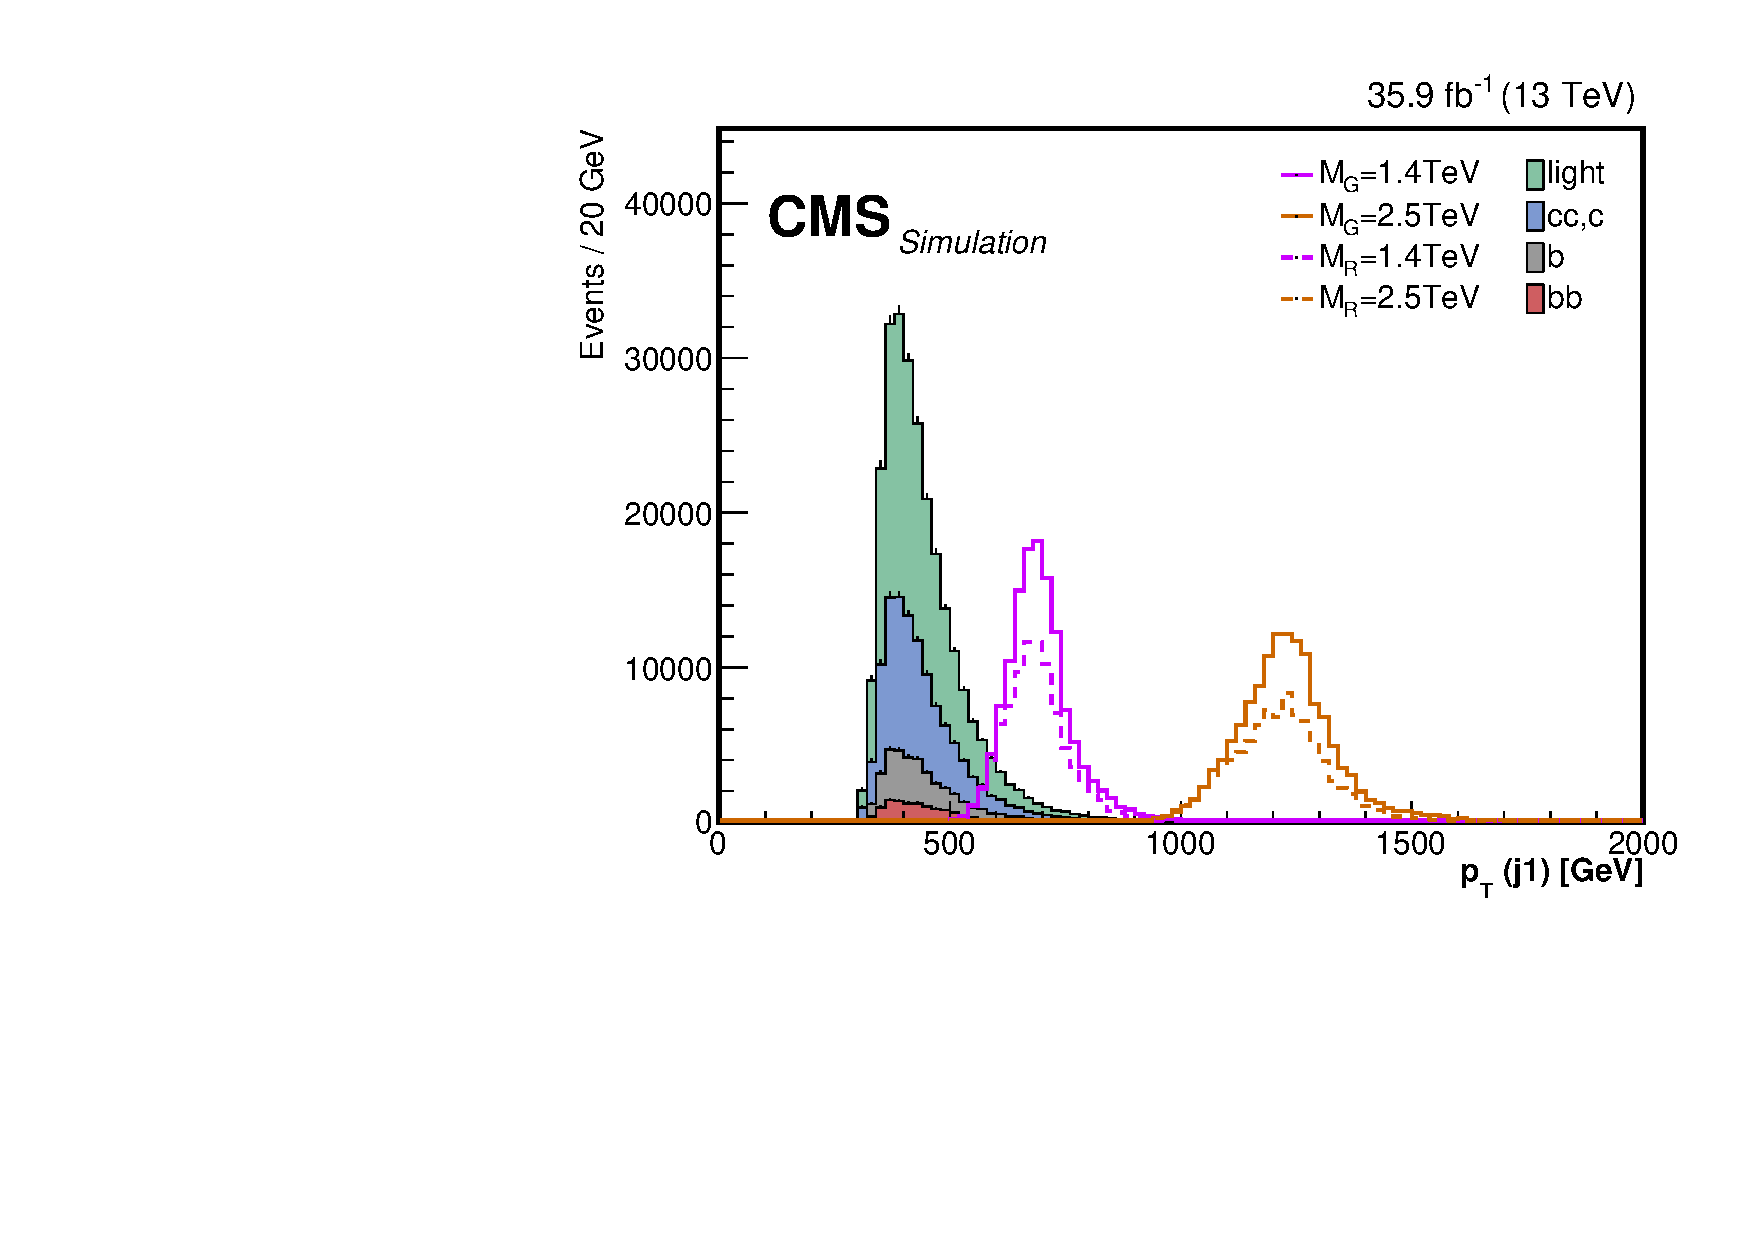
\includegraphics[width=0.5\textwidth]{Figures/MC_N1/pt_j0.pdf} &
    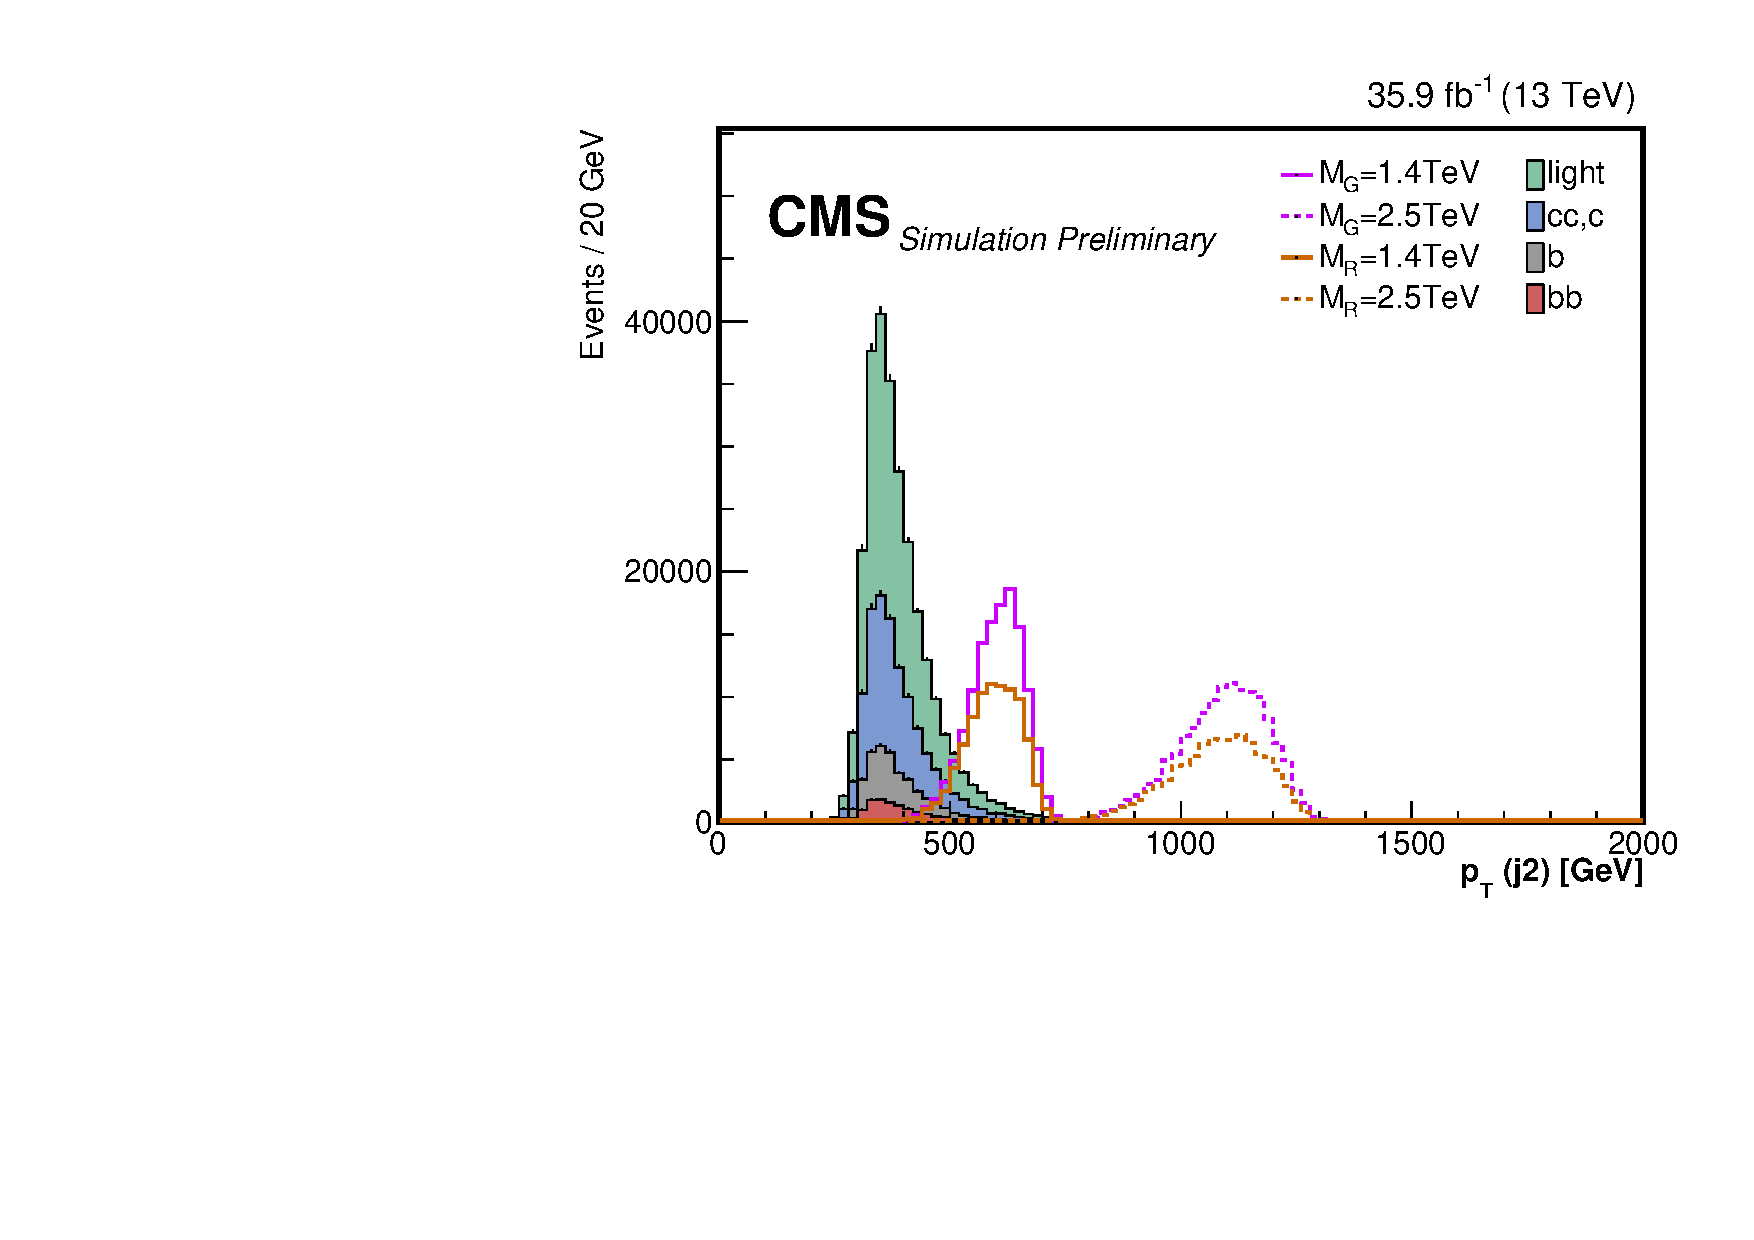
\includegraphics[width=0.5\textwidth]{Figures/MC_N1/pt_j1.pdf} \\
     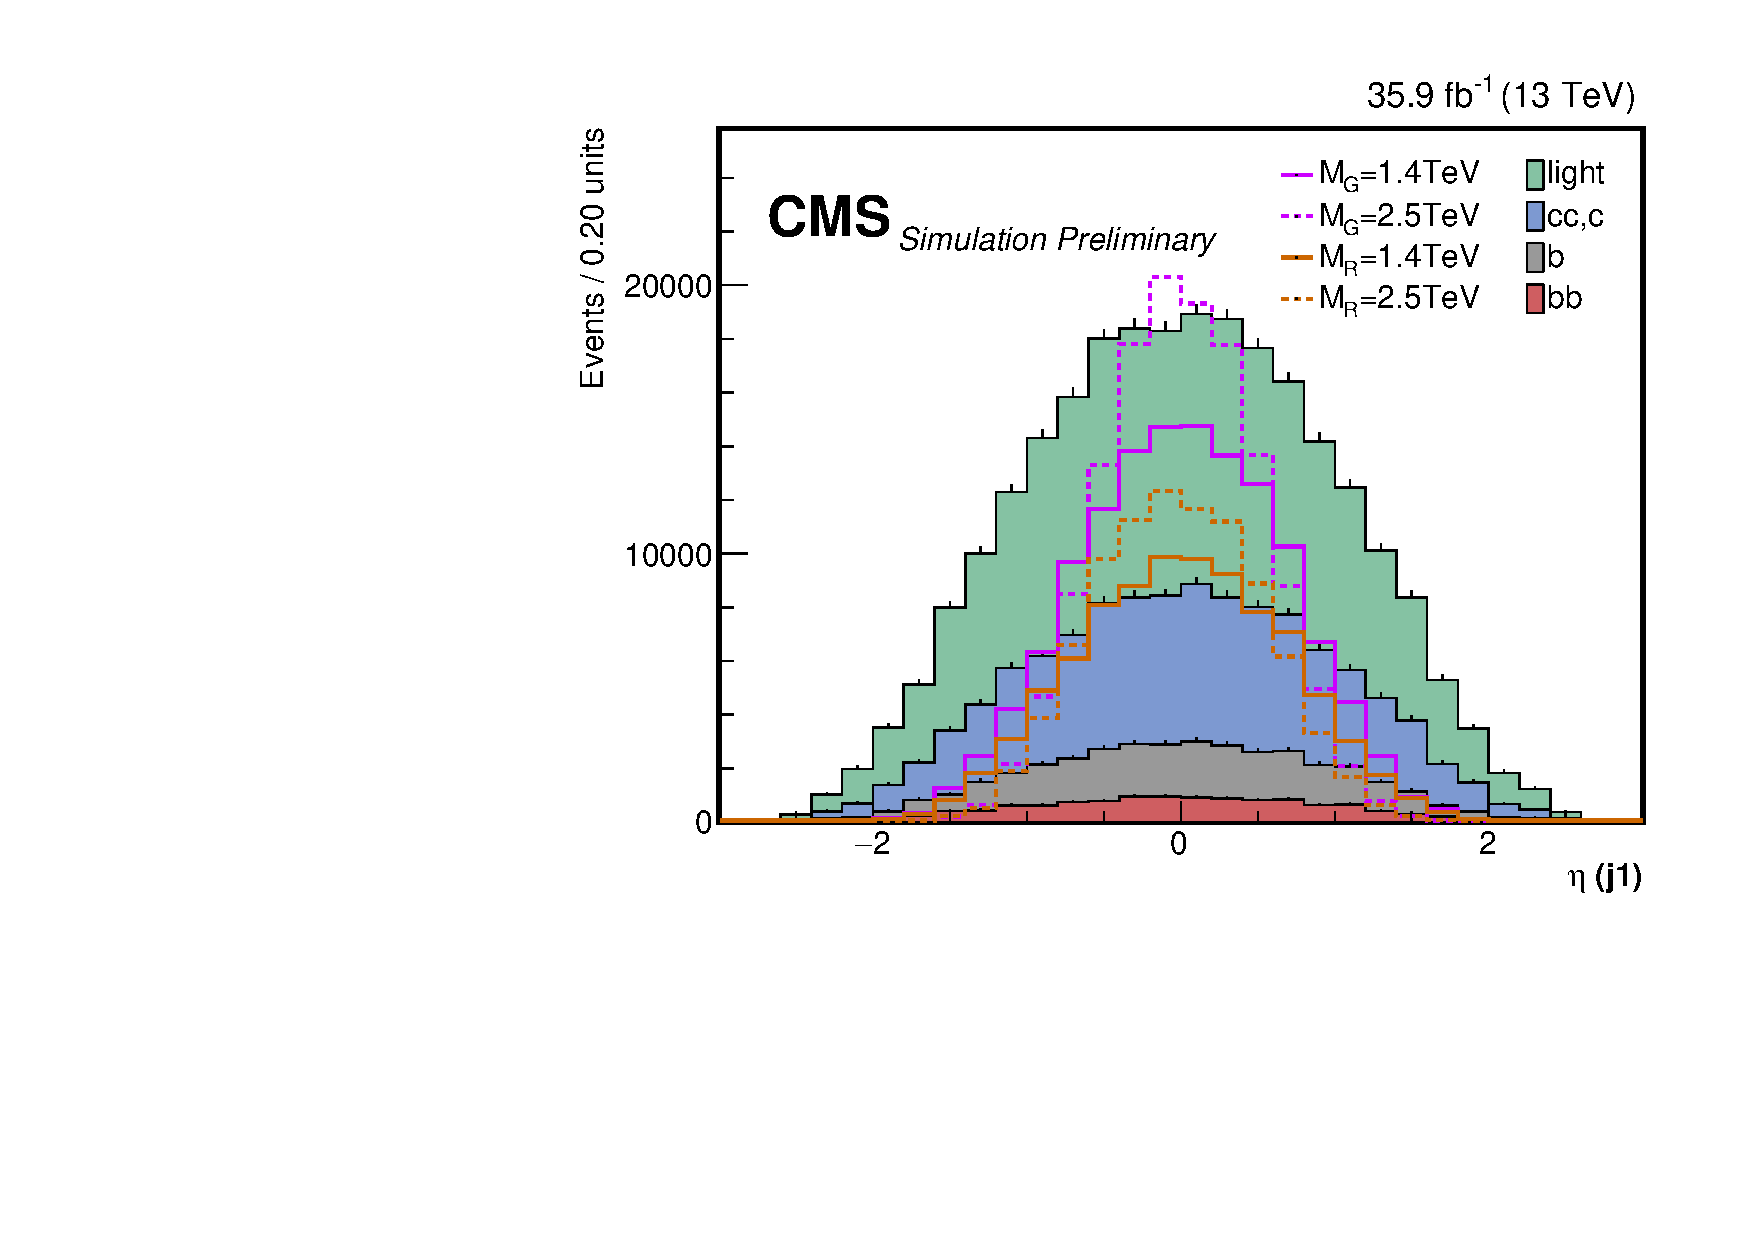
\includegraphics[width=0.5\textwidth]{Figures/MC_N1/eta_j0.pdf} &
    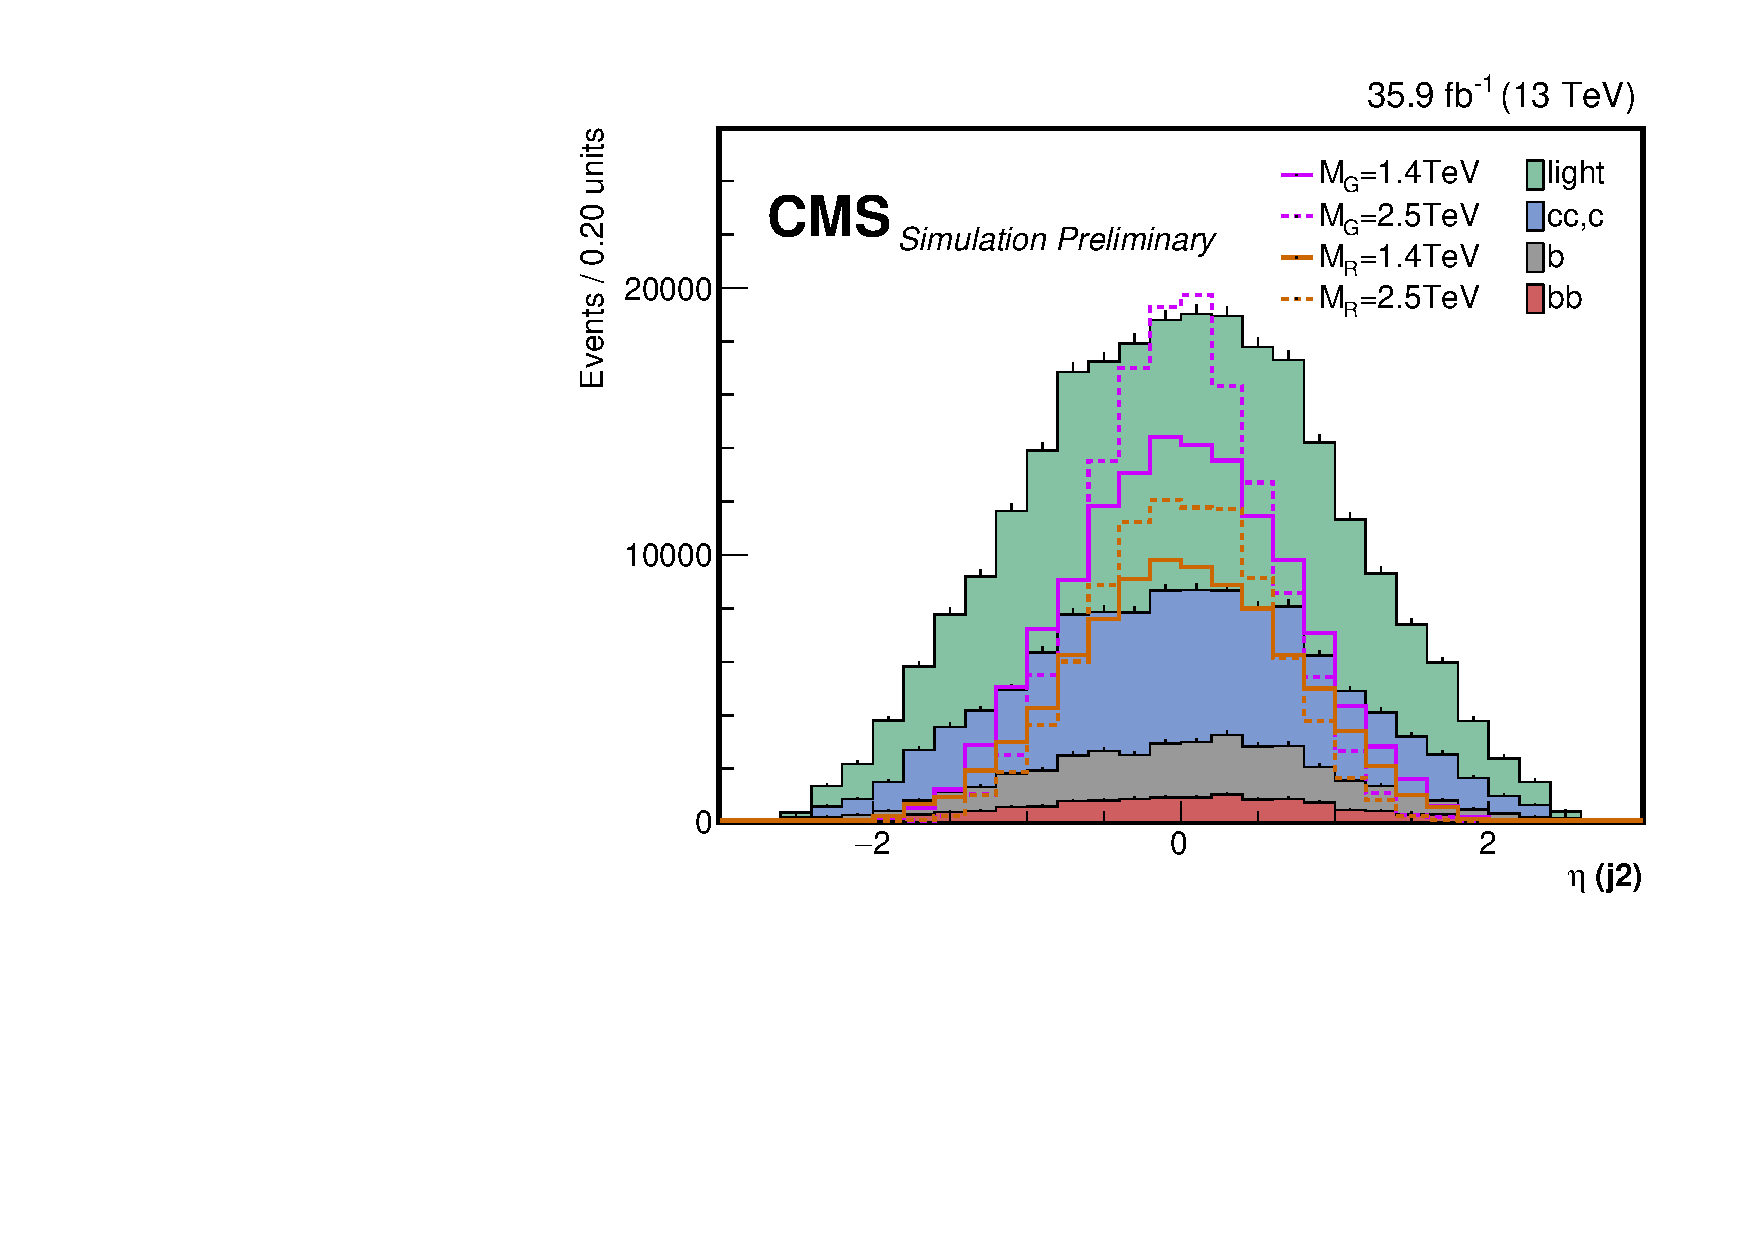
\includegraphics[width=0.5\textwidth]{Figures/MC_N1/eta_j1.pdf} \\
     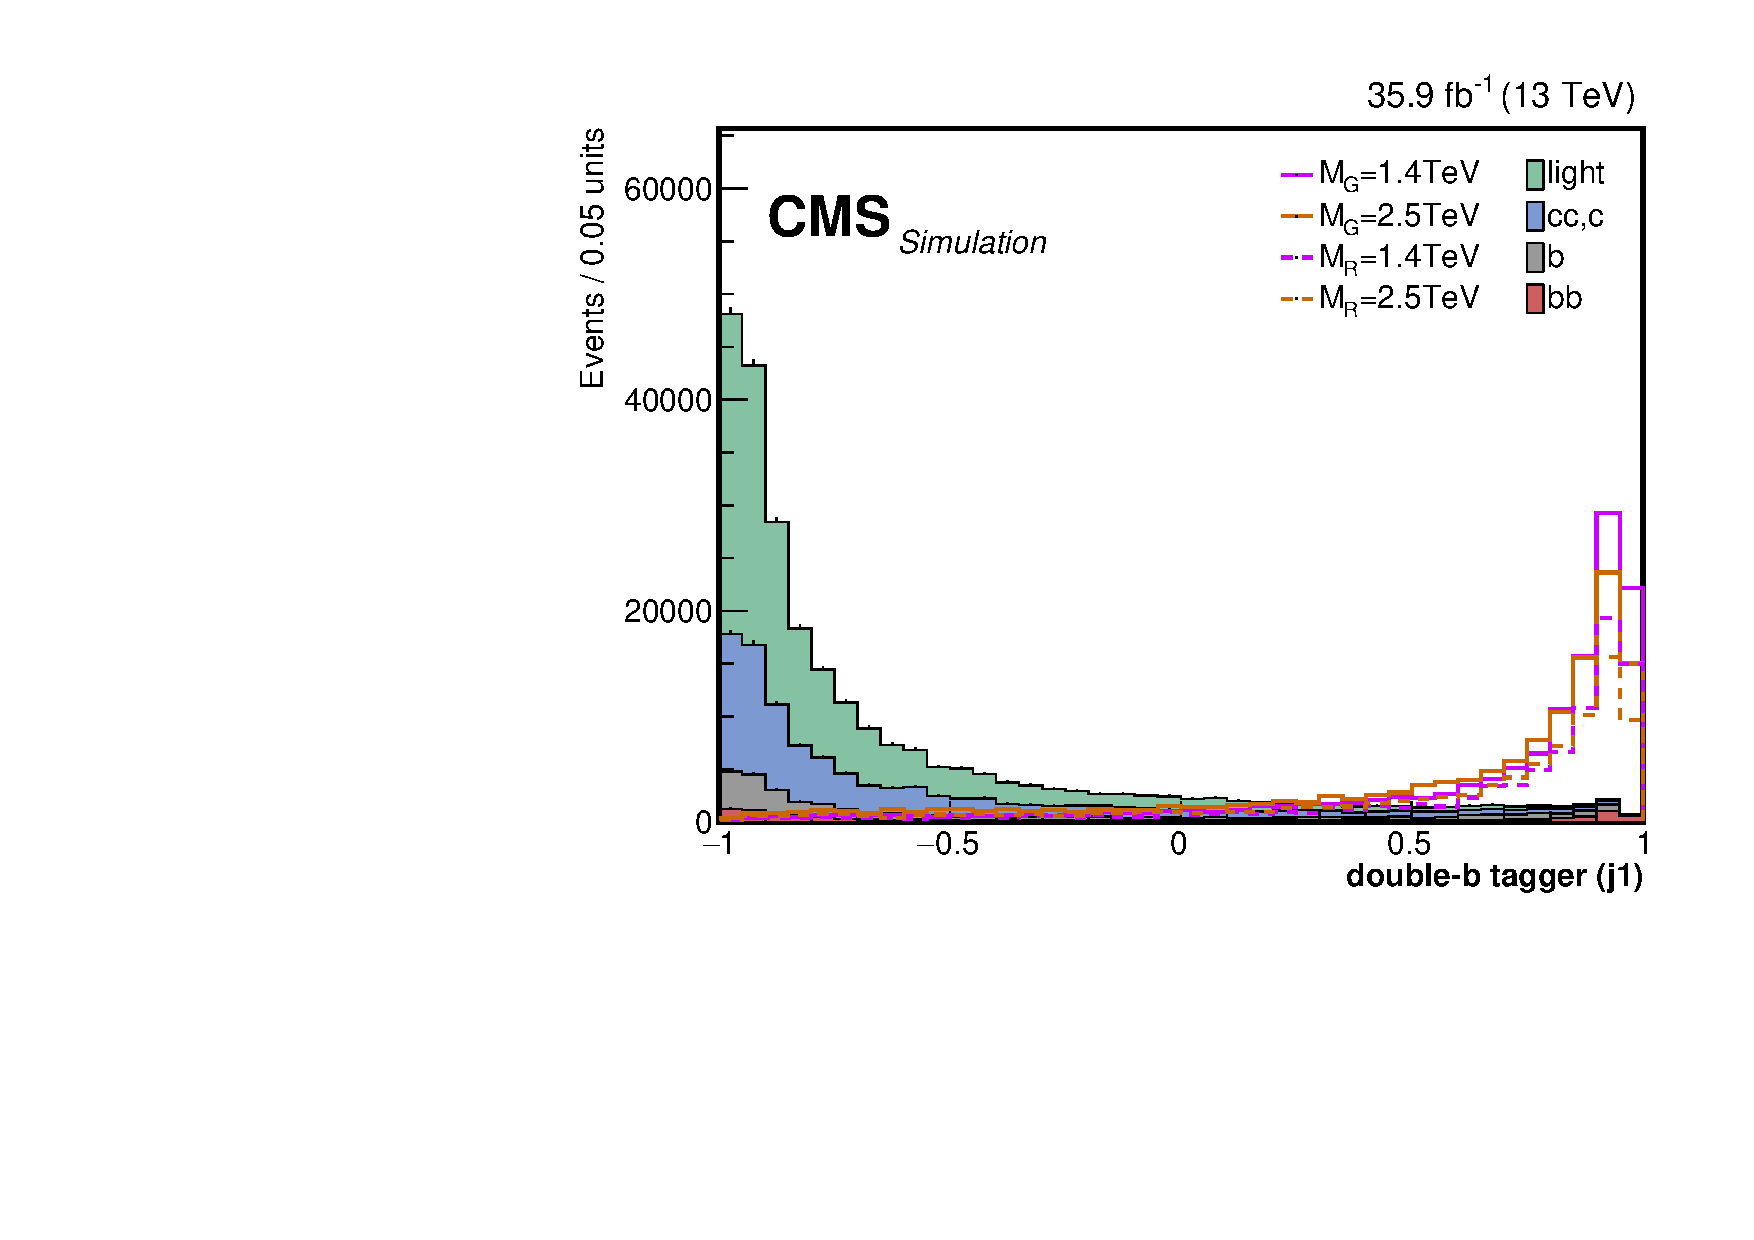
\includegraphics[width=0.5\textwidth]{Figures/MC_N1/doubleSV_j0.pdf} &
    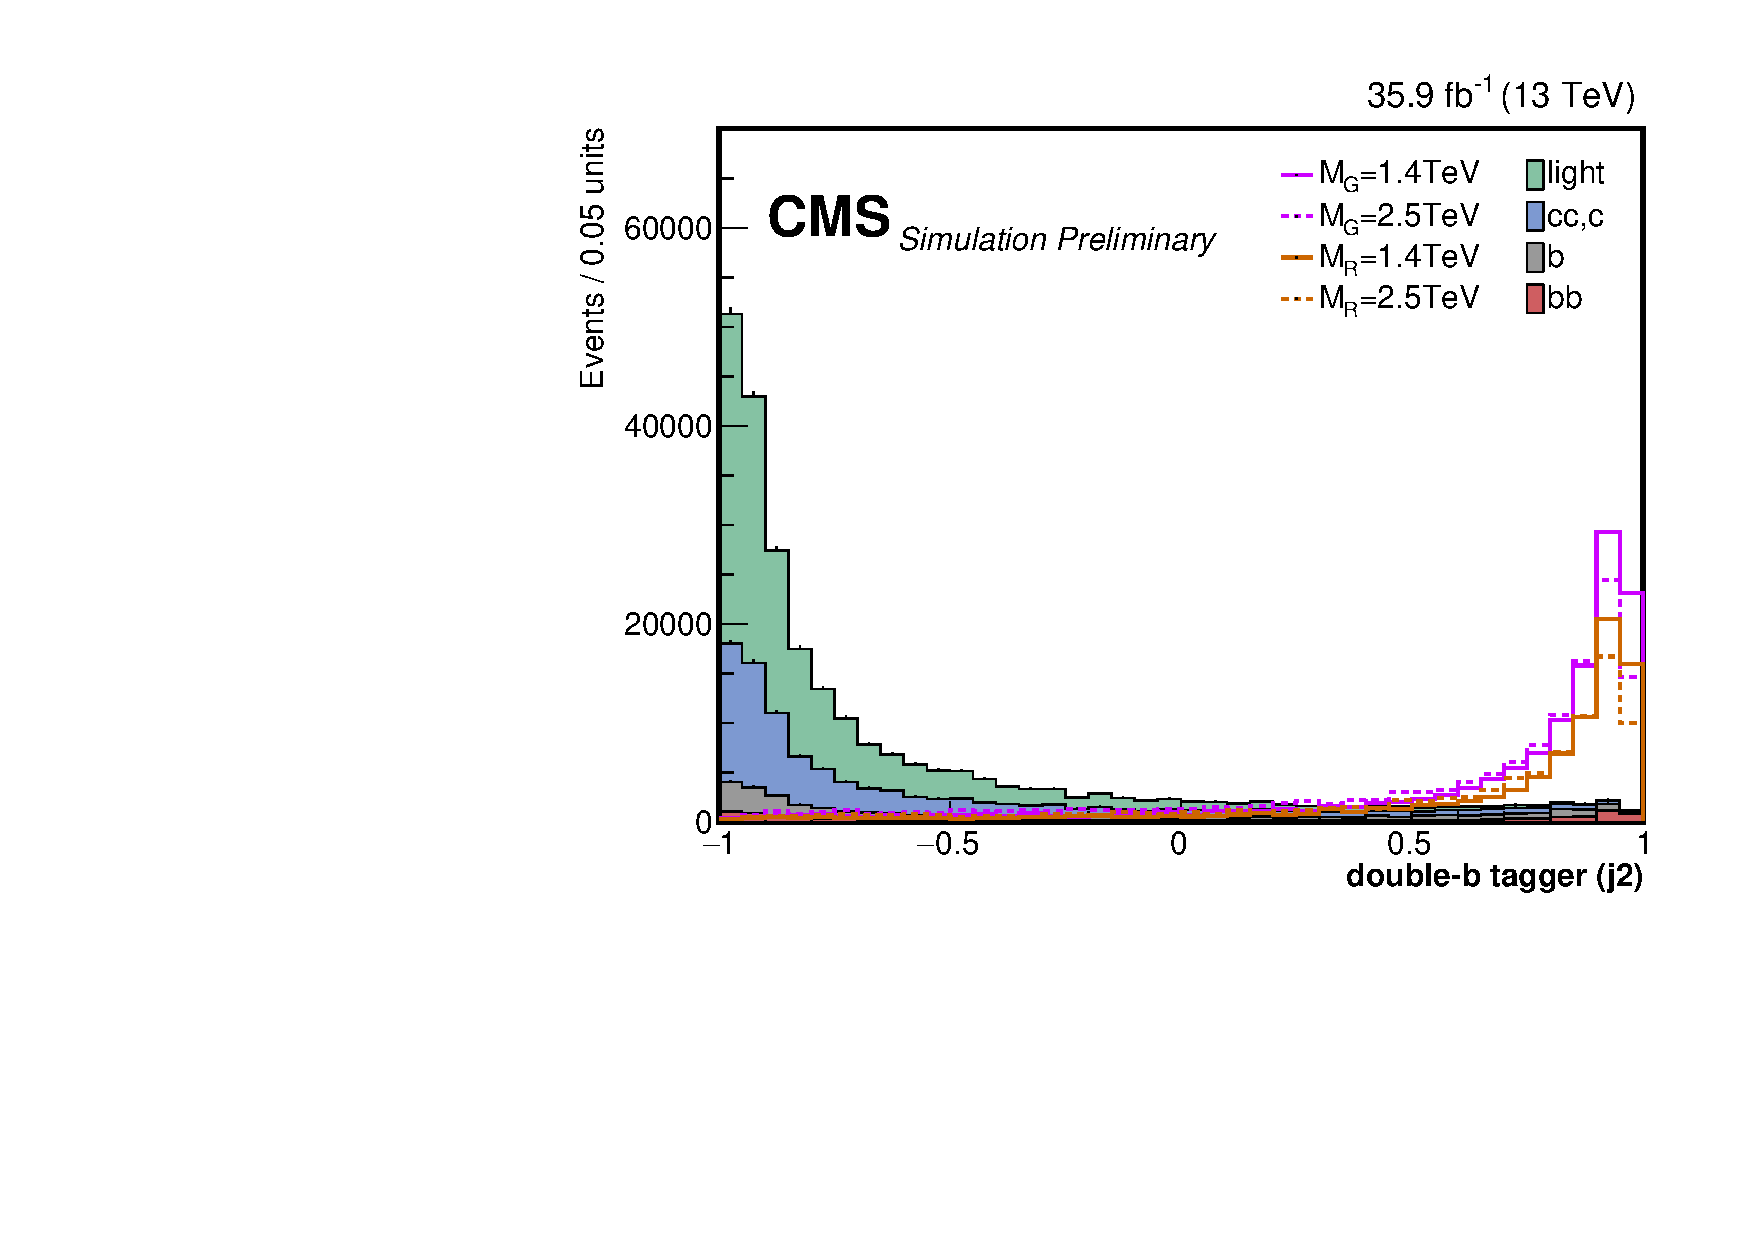
\includegraphics[width=0.5\textwidth]{Figures/MC_N1/doubleSV_j1.pdf} \\
  \end{tabular}
  \caption{Branching ratios as a function of the resonance mass for a W' (left) and Z' (right) in the HVT Minimal Composite Higgs Model.}
  \label{fig:hvt_brs}
\end{figure}

\begin{figure}[t]
  \centering
  \begin{tabular}{cc}
    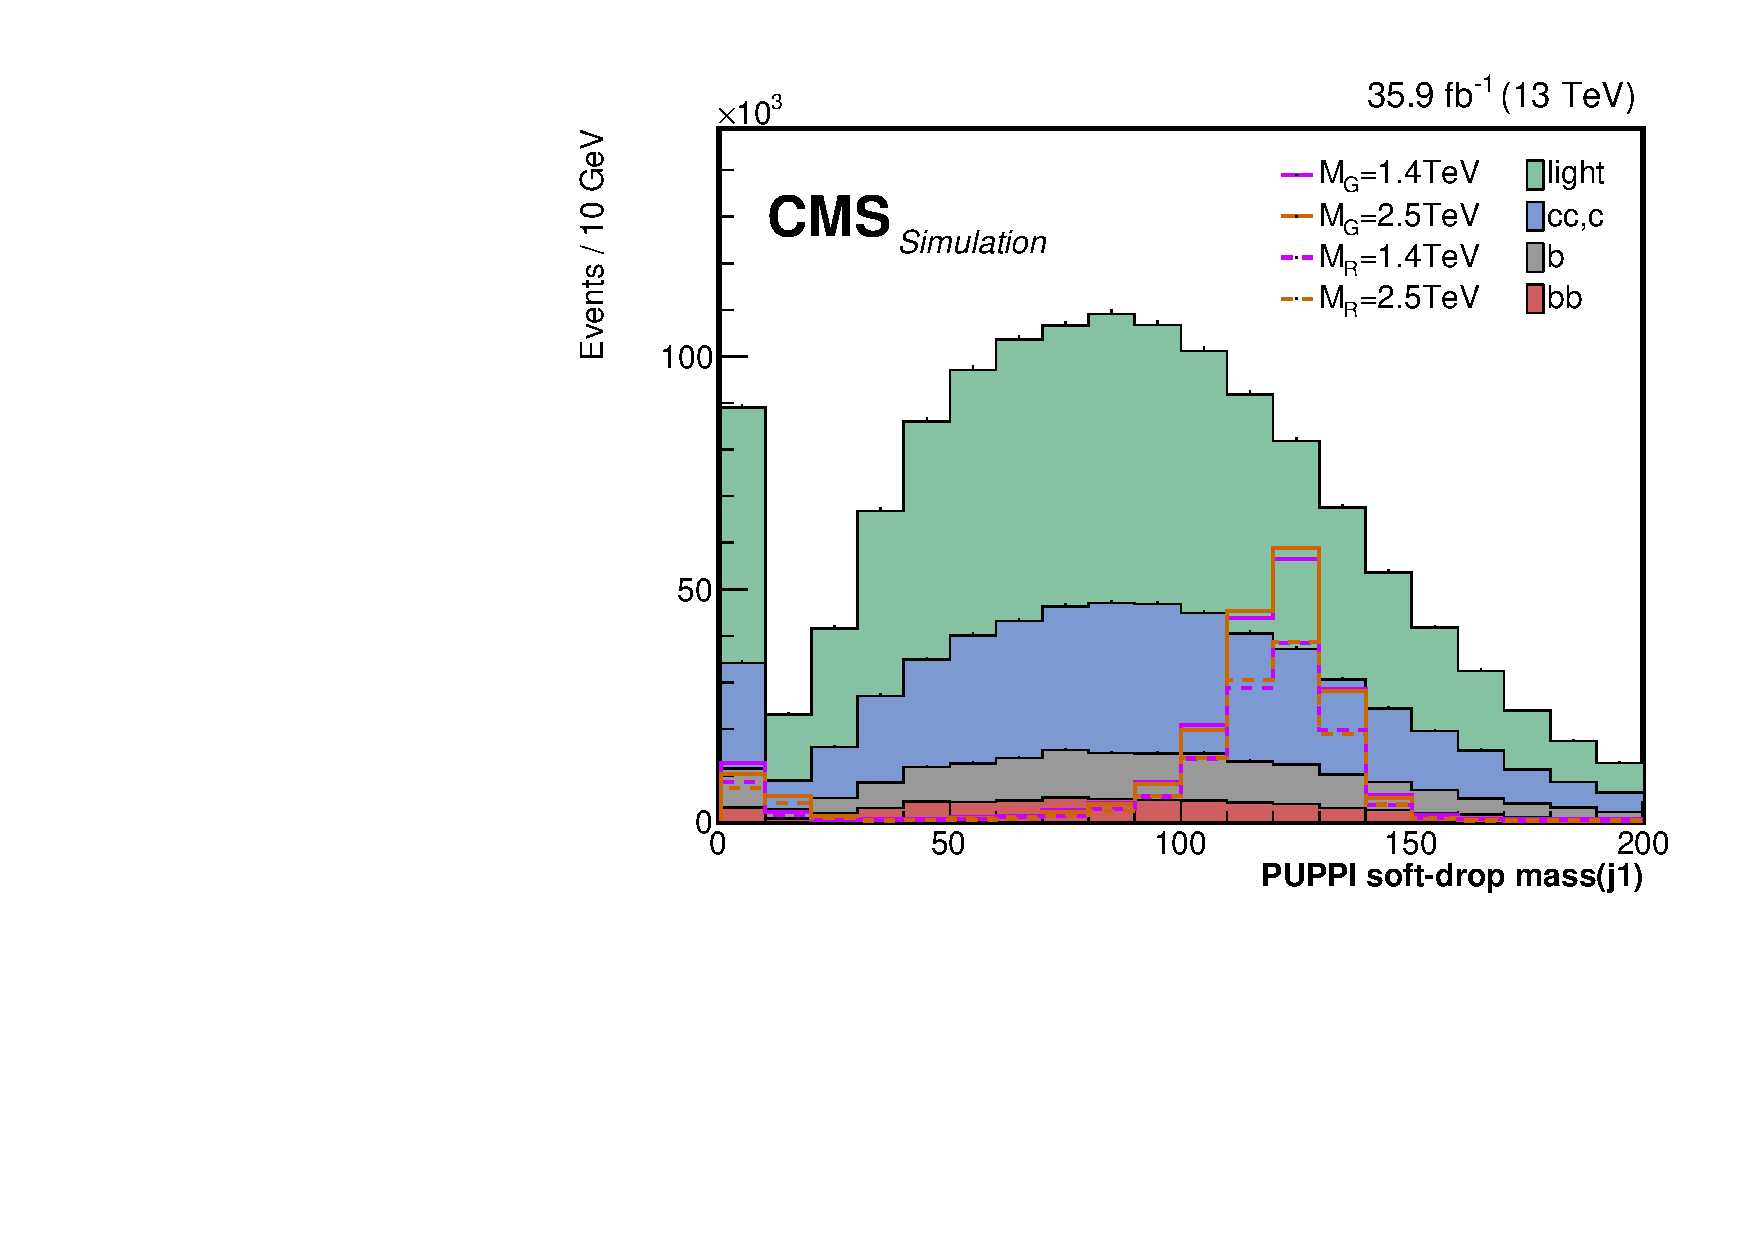
\includegraphics[width=0.5\textwidth]{Figures/MC_N1/puppiSDMassThea_j0.pdf} &
    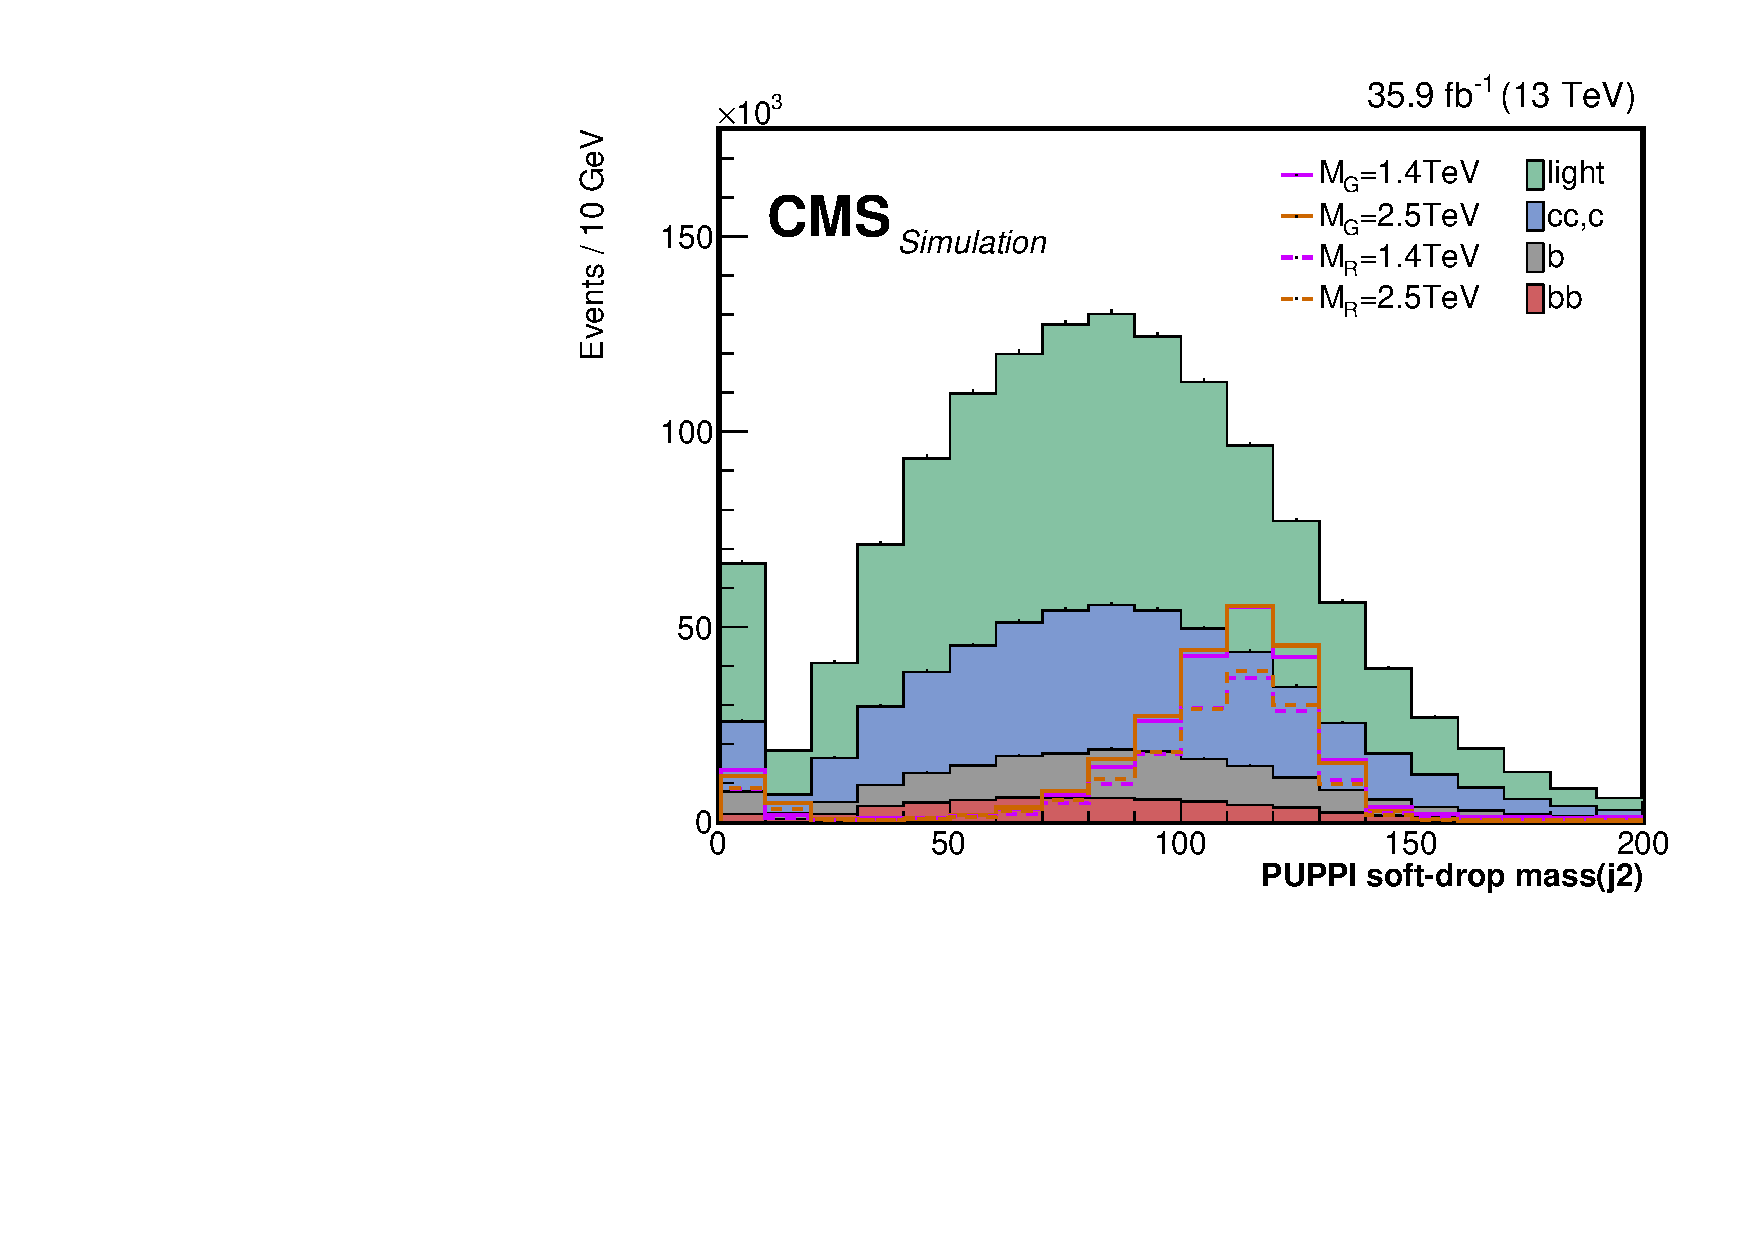
\includegraphics[width=0.5\textwidth]{Figures/MC_N1/puppiSDMassThea_j1.pdf} \\
     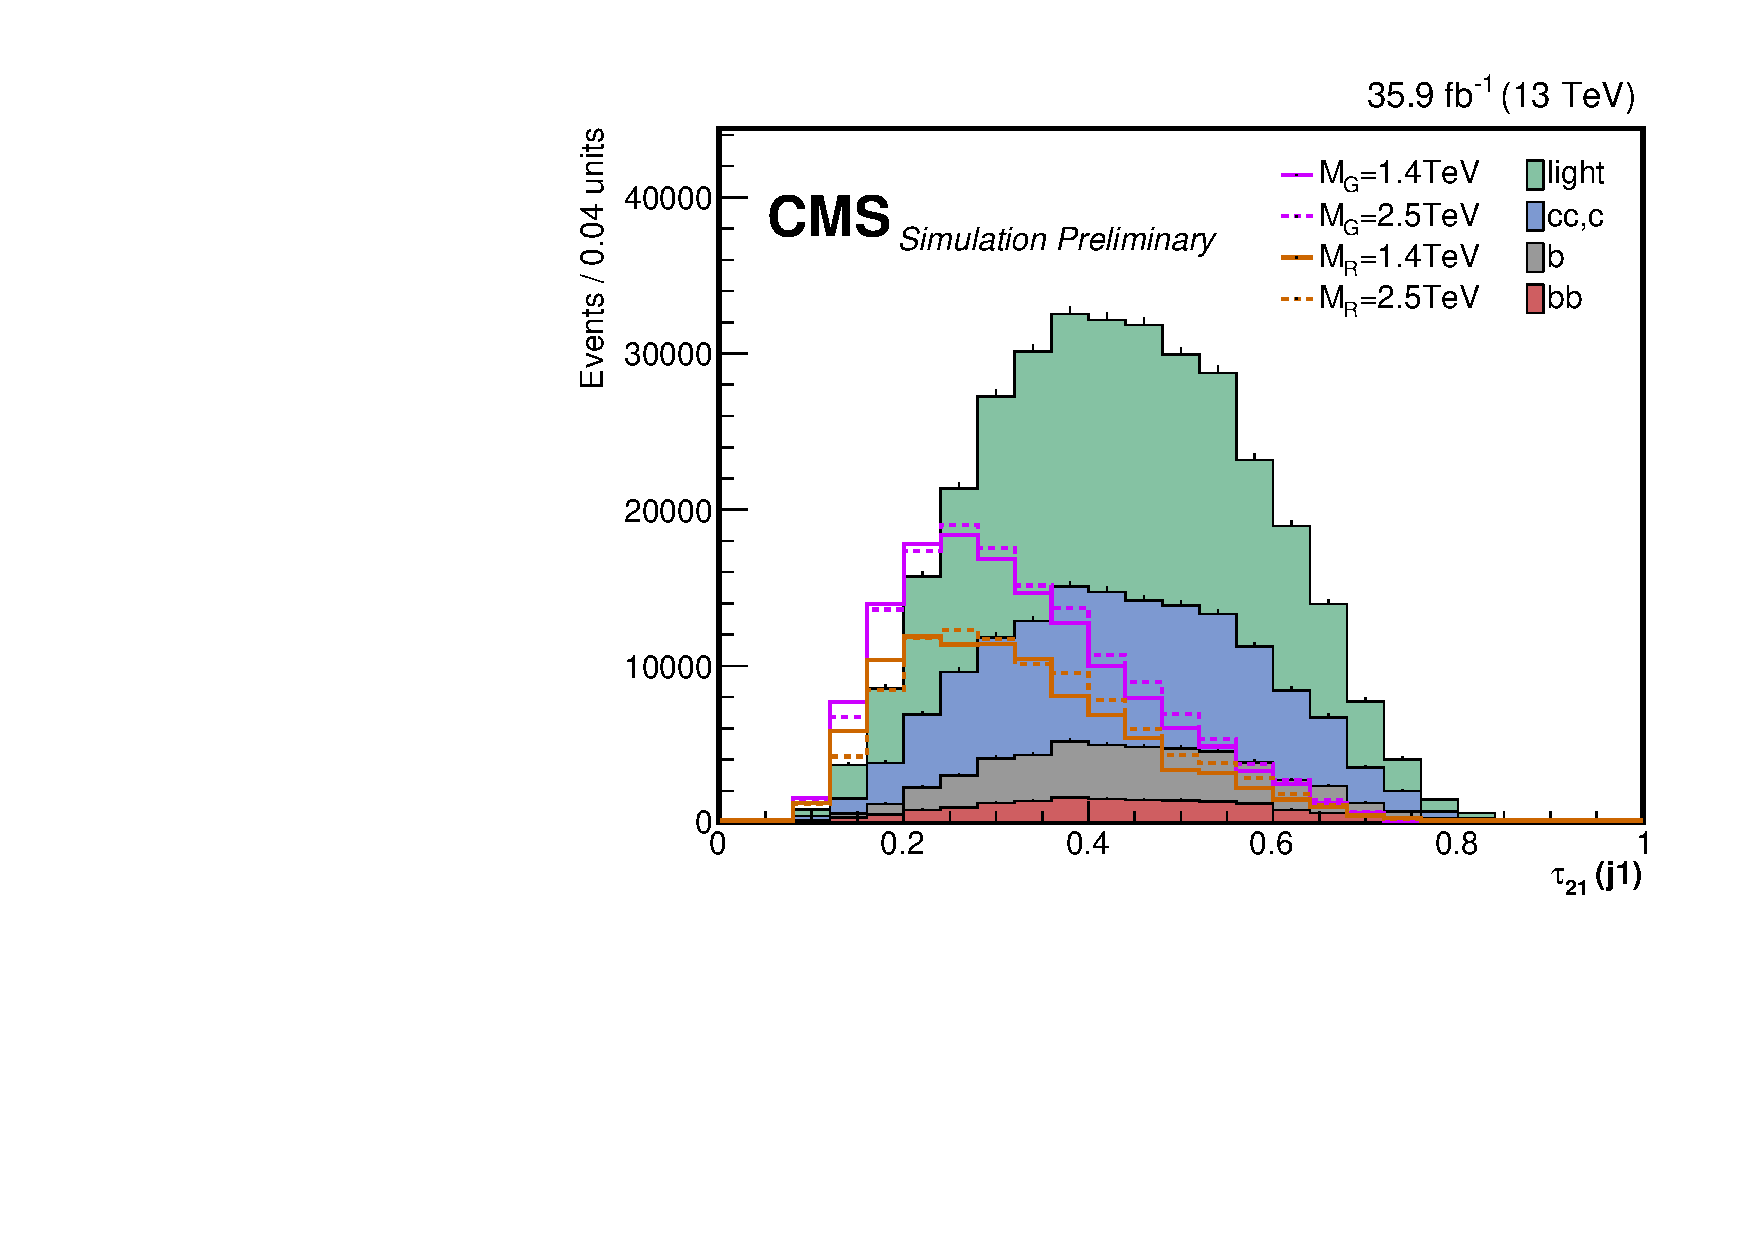
\includegraphics[width=0.5\textwidth]{Figures/MC_N1/puppiTau21_j0.pdf} &
    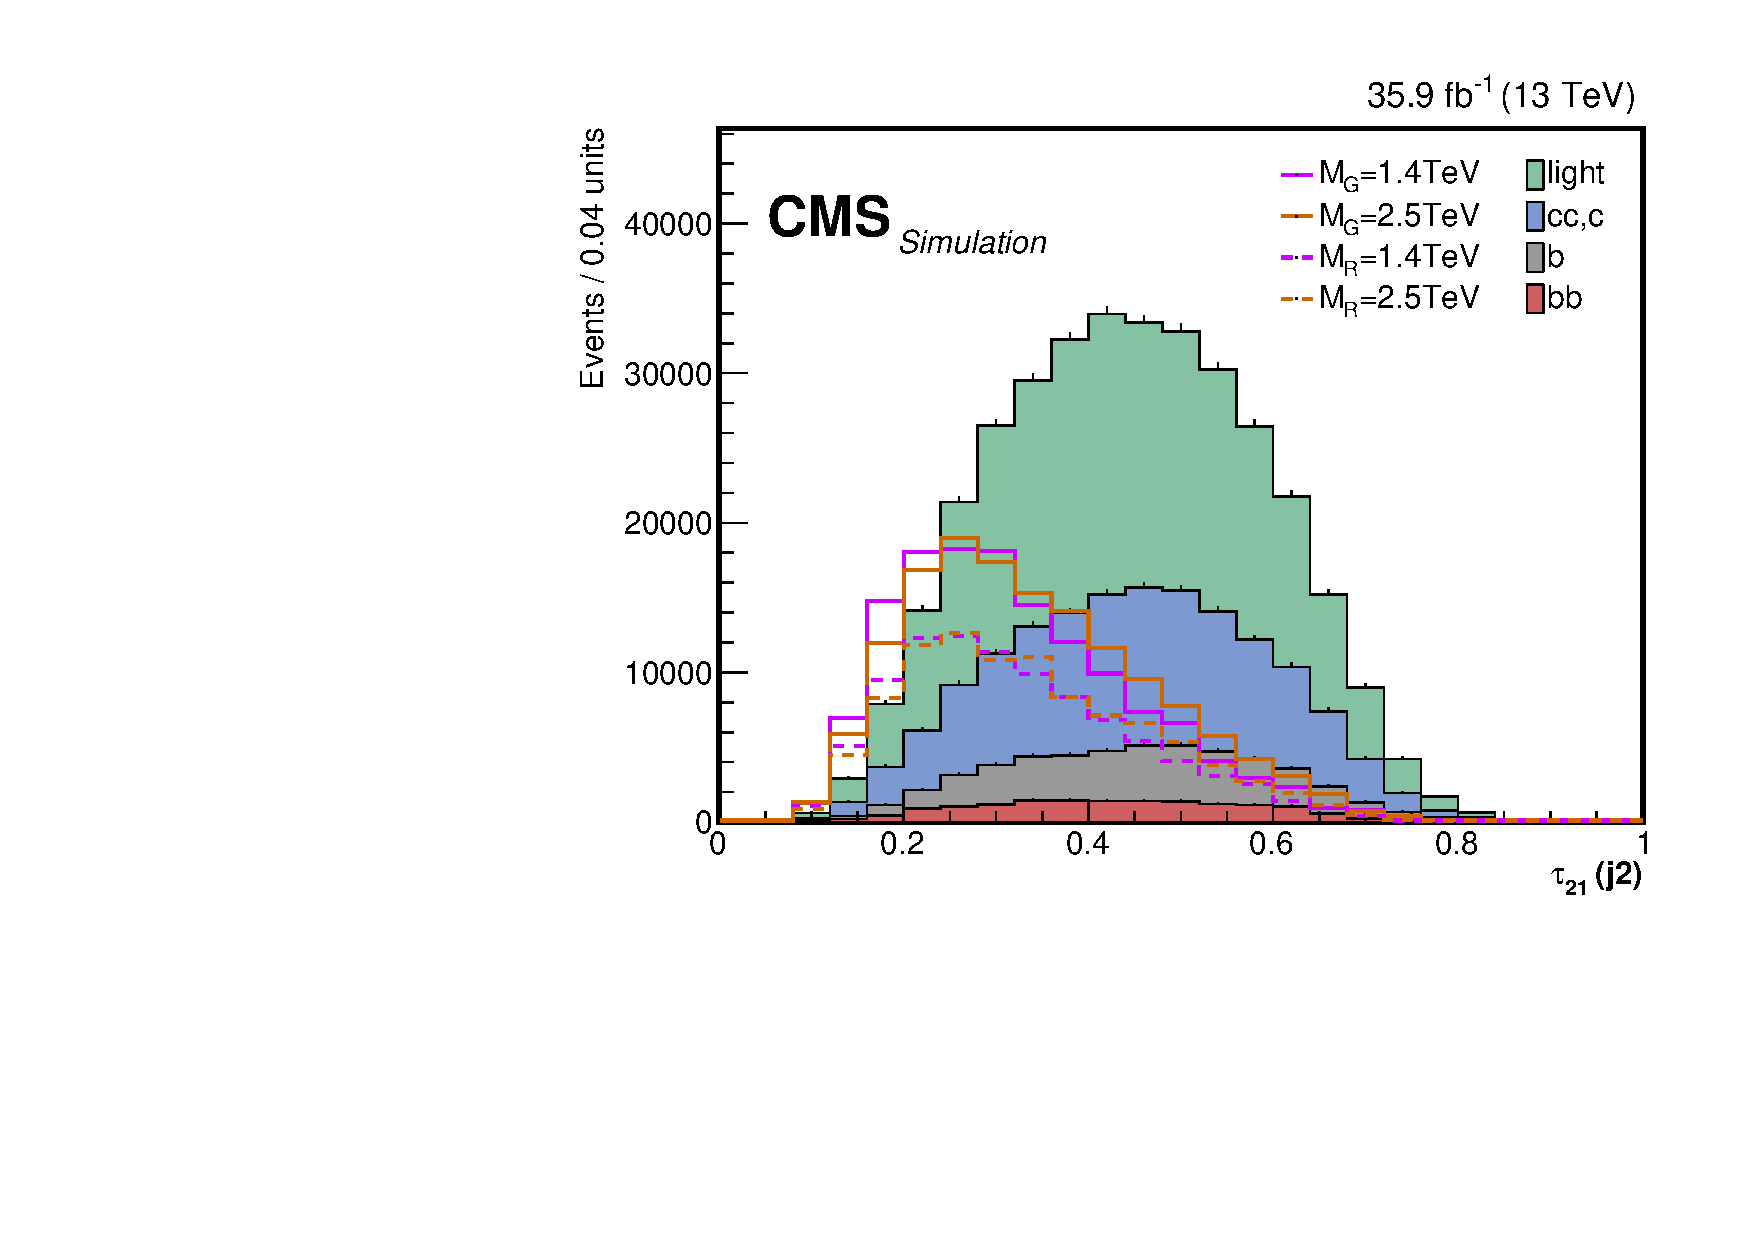
\includegraphics[width=0.5\textwidth]{Figures/MC_N1/puppiTau21_j1.pdf} \\
     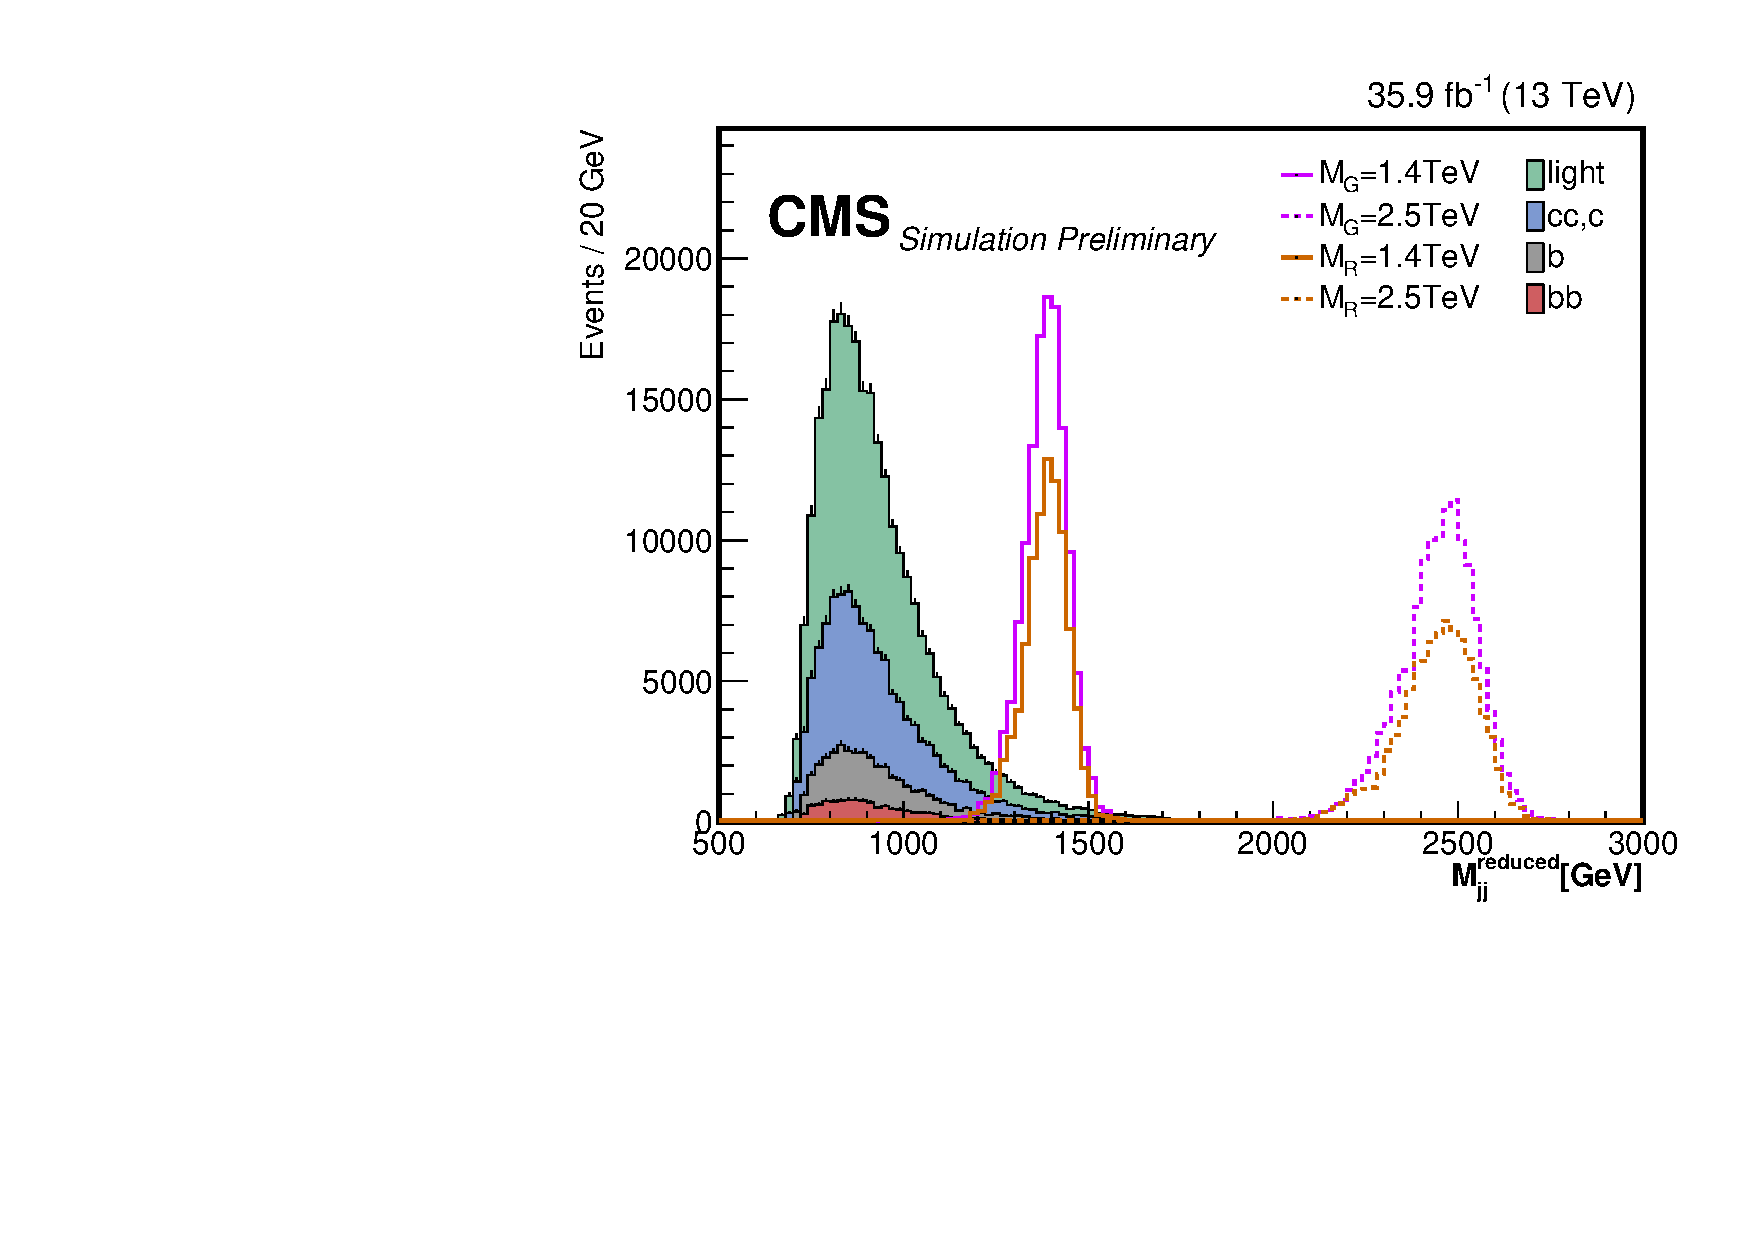
\includegraphics[width=0.5\textwidth]{Figures/MC_N1/totalMassRed.pdf} &
    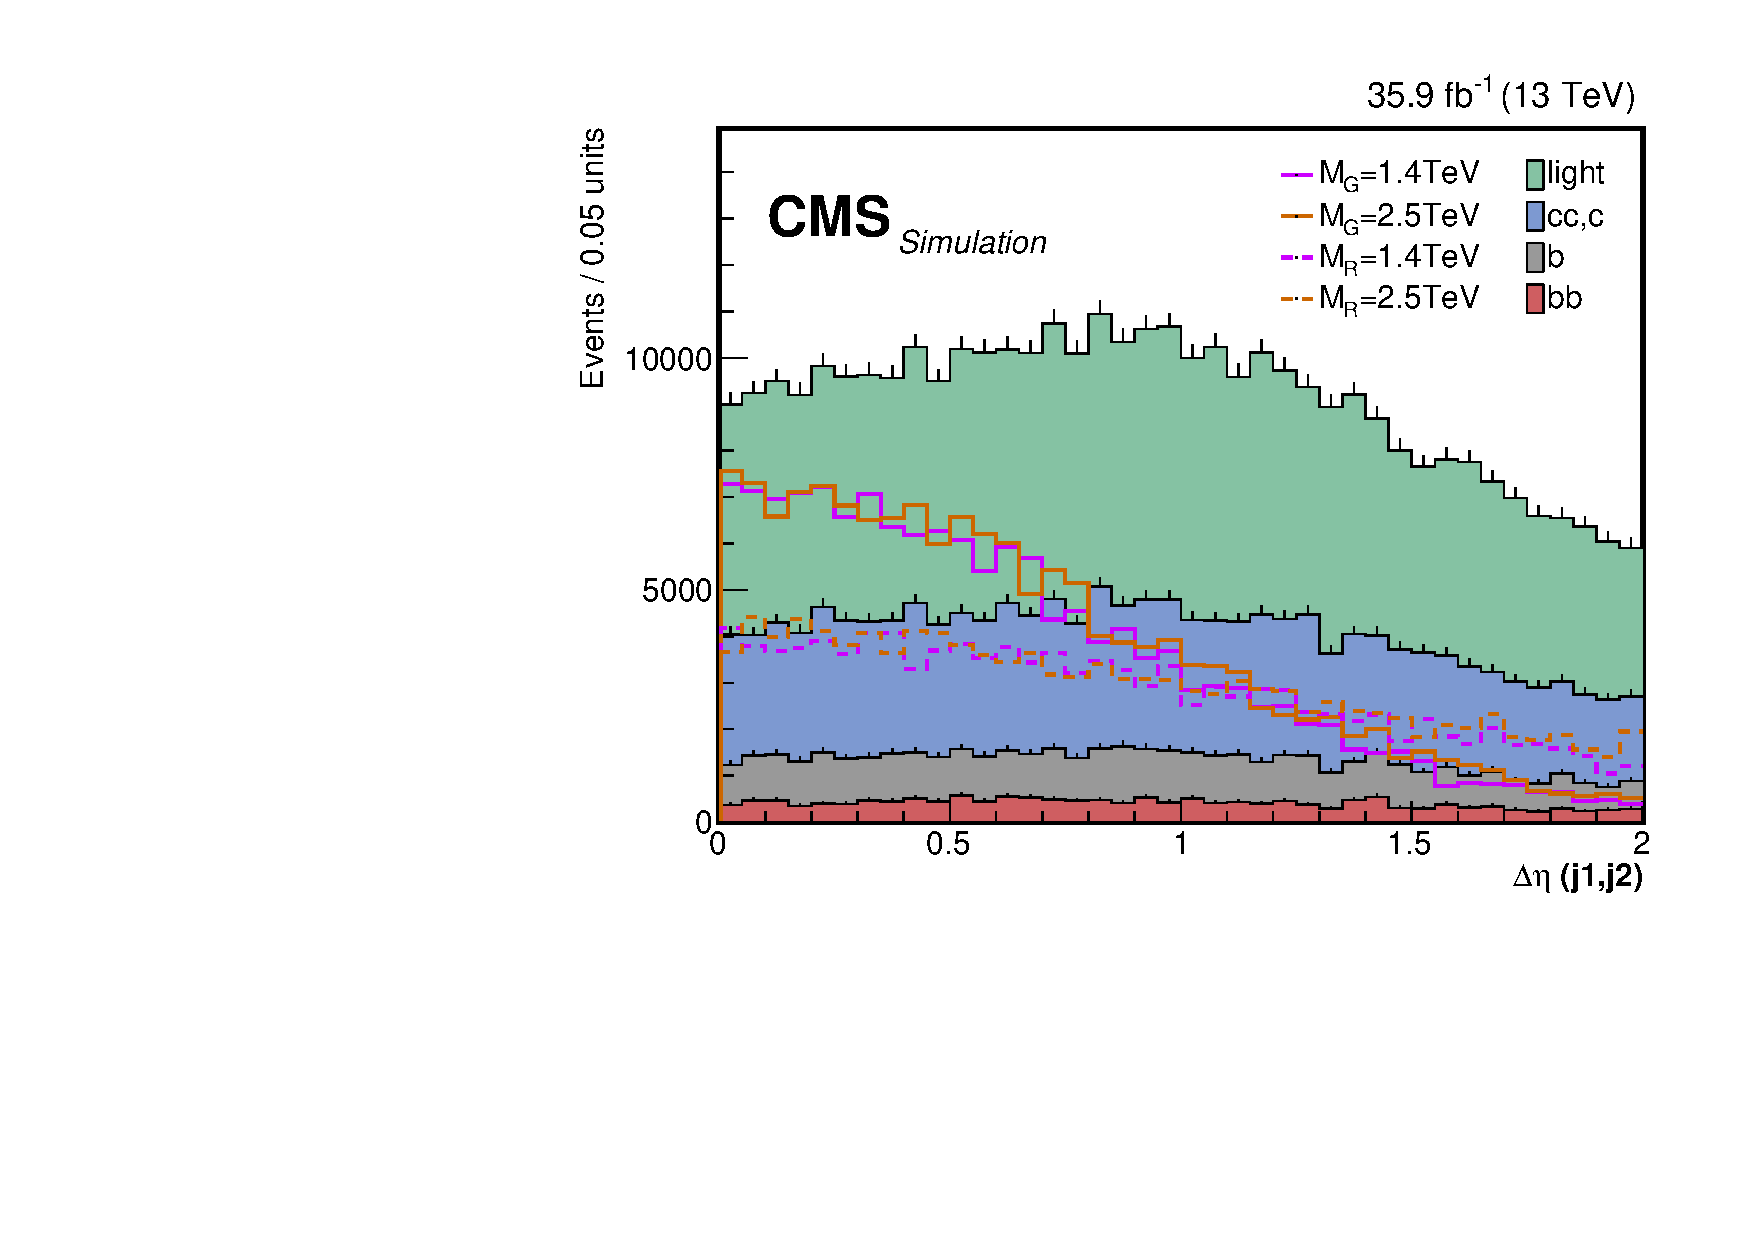
\includegraphics[width=0.5\textwidth]{Figures/MC_N1/deltaEta.pdf} \\
  \end{tabular}
  \caption{Branching ratios as a function of the resonance mass for a W' (left) and Z' (right) in the HVT Minimal Composite Higgs Model.}
  \label{fig:hvt_brs}
\end{figure}

